\chapter{Frey Microwave Auditory Effect}
\label{ch:frey-microwave-auditory-effect}

\begin{nontechnical}
\textbf{Imagine hearing sounds---clicks, buzzes, or even voices---without any speaker, headphones, or actual sound waves in the air.}

\textbf{The Frey effect makes this possible:} Rapid pulses of microwave energy (similar to radar) cause tiny, rapid heating in your head. This heating is so fast it creates pressure waves that travel to your inner ear, where they're detected as sound.

\textbf{Key points:}
\begin{itemize}
\item The ``sound'' is created \emph{inside your head}, not in the air
\item Someone standing next to you won't hear it
\item It's completely safe at typical exposure levels
\item Your cell phone cannot do this (wrong type of signal, too weak)
\end{itemize}

\textbf{Real use:} Discovered in the 1960s near radar installations. Potential applications include non-lethal deterrents and specialized communication systems, though ethical concerns remain.
\end{nontechnical}

\section{Overview}

The \textbf{Frey microwave auditory effect} (also known as \textbf{microwave hearing} or \textbf{RF hearing}) is the perception of auditory sensations when exposed to pulsed microwave radiation in the 1--10~GHz range. Remarkably, the effect occurs \textbf{without external sound waves}---the perception arises from \textbf{thermoelastic expansion} within brain tissue near the cochlea.

\begin{keyconcept}
The Frey effect requires \textbf{pulsed} microwave energy (not continuous wave). Each pulse causes rapid microscopic heating ($\Delta T \sim 10^{-6}$~K) that launches an acoustic pressure wave detectable by the inner ear. The perceived sound frequency matches the \textbf{pulse repetition rate}, not the microwave carrier frequency.
\end{keyconcept}

\textbf{Key characteristics:}
\begin{itemize}
\item \textbf{Pulse requirement:} Continuous-wave (CW) microwaves are ineffective
\item \textbf{Perceived frequency:} Determined by pulse repetition rate (10~Hz to 20~kHz)
\item \textbf{Energy threshold:} $\sim$1--10~$\mu$J/cm$^2$ per pulse (extremely low)
\item \textbf{Mechanism:} Thermoelastic transduction: EM $\rightarrow$ heat $\rightarrow$ pressure $\rightarrow$ neural signal
\item \textbf{Cochlear dependency:} Effect requires intact cochlea (hair cells)
\end{itemize}



\section{Discovery and Historical Background}

\subsection{Allan Frey's Original Experiments (1962)}

In 1962, Allan Frey at General Electric's Advanced Electronics Center reported an unusual phenomenon: personnel near radar installations heard ``clicking'' or ``buzzing'' sounds synchronized with radar pulses---despite no detectable airborne sound.

\textbf{Controlled laboratory experiments:}
\begin{itemize}
\item \textbf{Parameters:} 1.3~GHz carrier, $\sim$10~$\mu$s pulse width, 100--1000~pps
\item \textbf{Key observation:} Auditory perception reported even in \emph{deaf subjects} with conductive hearing loss (middle ear damage)
\item \textbf{Sensorineural deaf:} Individuals with cochlear damage perceived nothing
\item \textbf{Localization:} Sound appeared to originate inside the head, not from external space
\end{itemize}

\textbf{Frey's conclusion:} Microwaves directly stimulate the auditory system, bypassing the external and middle ear but requiring an intact cochlea.

\begin{calloutbox}{Initial Skepticism}
The effect was initially dismissed as electromagnetic interference with measurement equipment or neural tissue. However, independent replication by multiple laboratories in the 1970s confirmed the phenomenon was real and biological in origin.
\end{calloutbox}

\subsection{Subsequent Research (1970s--1990s)}

Following Frey's discovery, extensive research---much of it initially classified military studies---established the mechanism and parameters:

\textbf{Key experimental findings:}
\begin{itemize}
\item Effect requires \textbf{intact cochlea}; direct neural stimulation ruled out
\item Perceived frequency matches \textbf{pulse repetition rate}: 10~pps $\rightarrow$ 10~Hz tone
\item Peak sensitivity at $\sim$2.45~GHz (ISM band), where penetration and absorption are optimized
\item Threshold energy density: 1--10~$\mu$J/cm$^2$ per pulse
\item Effect occurs in multiple species (humans, cats, guinea pigs, rats)
\end{itemize}

\textbf{Theoretical breakthrough:} Lin and Foster (1974--1980) developed the \textbf{thermoelastic theory}, which quantitatively explained the effect and predicted experimental thresholds within a factor of 2--3.

\section{Mechanism: Thermoelastic Transduction}
\label{sec:frey-mechanism}

The Frey effect involves a five-stage energy conversion process:

\subsection{Physical Process}

\begin{center}
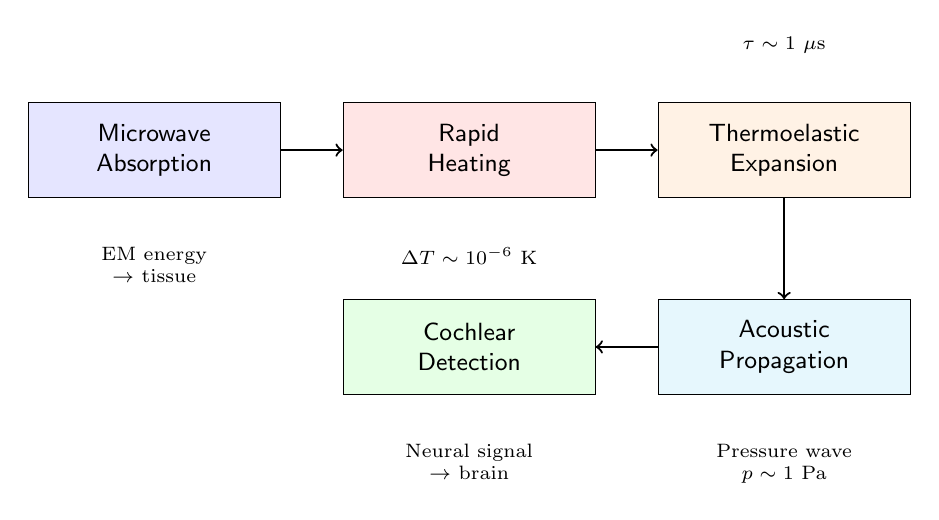
\begin{tikzpicture}[
  block/.style={rectangle, draw, minimum width=3.2cm, minimum height=1.2cm, font=\sffamily\small, align=center},
  node distance=2cm,
  font=\small
]
\node[block, fill=blue!10] (absorb) {Microwave\\Absorption};
\node[block, fill=red!10, right of=absorb, node distance=4cm] (heat) {Rapid\\Heating};
\node[block, fill=orange!10, right of=heat, node distance=4cm] (expand) {Thermoelastic\\Expansion};
\node[block, fill=cyan!10, below of=expand, node distance=2.5cm] (acoustic) {Acoustic\\Propagation};
\node[block, fill=green!10, left of=acoustic, node distance=4cm] (perception) {Cochlear\\Detection};

\draw[->,thick] (absorb) -- (heat);
\draw[->,thick] (heat) -- (expand);
\draw[->,thick] (expand) -- (acoustic);
\draw[->,thick] (acoustic) -- (perception);

\node[below=0.5cm, font=\scriptsize, align=center] at (absorb.south) {EM energy\\$\rightarrow$ tissue};
\node[below=0.5cm, font=\scriptsize, align=center] at (heat.south) {$\Delta T \sim 10^{-6}$~K};
\node[above=0.5cm, font=\scriptsize, align=center] at (expand.north) {$\tau \sim 1$~$\mu$s};
\node[below=0.5cm, font=\scriptsize, align=center] at (acoustic.south) {Pressure wave\\$p \sim 1$~Pa};
\node[below=0.5cm, font=\scriptsize, align=center] at (perception.south) {Neural signal\\$\rightarrow$ brain};
\end{tikzpicture}
\end{center}

\textbf{Step 1: Microwave Absorption}

Pulsed microwave energy is absorbed primarily by water molecules in brain tissue.
\begin{equation}
\text{Penetration depth:} \quad \delta = \frac{1}{\alpha} \approx 1\text{--}3~\text{cm at 1--10~GHz}
\label{eq:frey-penetration}
\end{equation}
where $\alpha$ is the absorption coefficient (Np/m).

\textbf{Step 2: Rapid Heating}

The absorbed energy causes localized temperature rise:
\begin{equation}
\Delta T = \frac{\text{SAR} \cdot \tau}{c_p}
\label{eq:frey-temp-rise}
\end{equation}
where:
\begin{itemize}
\item $\text{SAR}$ = specific absorption rate (W/kg)
\item $\tau$ = pulse duration (typically 1--10~$\mu$s)
\item $c_p \approx 3600$~J/(kg$\cdot$K) = specific heat capacity of tissue
\end{itemize}

\textbf{Key requirement:} Pulse duration must be shorter than thermal diffusion time ($\sim$1~ms) to prevent heat spreading.

\textbf{Step 3: Thermoelastic Expansion}

Rapid heating causes tissue to expand before heat can diffuse:
\begin{equation}
\frac{\Delta V}{V} = 3\alpha_T \Delta T
\label{eq:frey-expansion}
\end{equation}
where $\alpha_T \approx 3 \times 10^{-4}$~K$^{-1}$ is the thermal expansion coefficient of tissue.

This expansion launches an acoustic pressure wave:
\begin{equation}
p = \frac{\beta}{\rho_0 c_p} \cdot \text{SAR} \cdot \tau \cdot f_c
\label{eq:frey-pressure}
\end{equation}
where:
\begin{itemize}
\item $\beta \approx 10^{-4}$~K$^{-1}$ = volumetric thermal expansion
\item $\rho_0 \approx 1000$~kg/m$^3$ = tissue density
\item $f_c$ = microwave carrier frequency (Hz)
\end{itemize}

\textbf{Step 4: Acoustic Propagation}

The pressure wave propagates through tissue at the speed of sound ($c_s \approx 1500$~m/s) to the cochlea.

\textbf{Step 5: Cochlear Detection}

Inner ear hair cells (stereocilia) respond to pressure variations, generating neural signals processed by the auditory cortex as sound.

\subsection{Quantitative Analysis}

\subsubsection{Energy and Temperature Calculations}

For a typical threshold-level pulse:
\begin{itemize}
\item Energy fluence: $E_f \approx 5$~$\mu$J/cm$^2$ per pulse
\item Pulse duration: $\tau = 1$~$\mu$s
\item SAR: $\sim$1~W/kg (localized)
\end{itemize}

Temperature rise per pulse:
\begin{equation}
\Delta T = \frac{\text{SAR} \cdot \tau}{c_p} = \frac{1 \times 10^{-6}}{3600} \approx 3 \times 10^{-10}~\text{K}
\label{eq:frey-temp-calc}
\end{equation}

\begin{calloutbox}{Negligible Thermal Effect}
The temperature rise is \textbf{ten million times smaller} than 1°C. The effect is not thermal damage but rather \textbf{thermoelastic transduction}---converting heat expansion into mechanical pressure.
\end{calloutbox}

\subsubsection{Pressure Wave Amplitude}

Using the Lin-Wang thermoelastic model with typical parameters:
\begin{equation}
p = \frac{\beta}{\rho_0 c_p} \cdot \text{SAR} \cdot \tau \cdot f_c
\label{eq:frey-pressure-calc}
\end{equation}

For $f_c = 2.45$~GHz (ISM band):
\begin{equation}
p \approx \frac{10^{-4}}{(1000)(3600)} \times 1 \times 10^{-6} \times 2.45 \times 10^9 \approx 0.07~\text{Pa}
\end{equation}

Converting to sound pressure level (SPL):
\begin{equation}
\text{SPL} = 20\log_{10}\left(\frac{p}{p_{\text{ref}}}\right) = 20\log_{10}\left(\frac{0.07}{20 \times 10^{-6}}\right) \approx 71~\text{dB SPL}
\end{equation}

This corresponds to \textbf{moderate loudness}---comparable to normal conversation.

\subsection{Why Pulsed Microwaves, Not Continuous Wave?}

\begin{center}
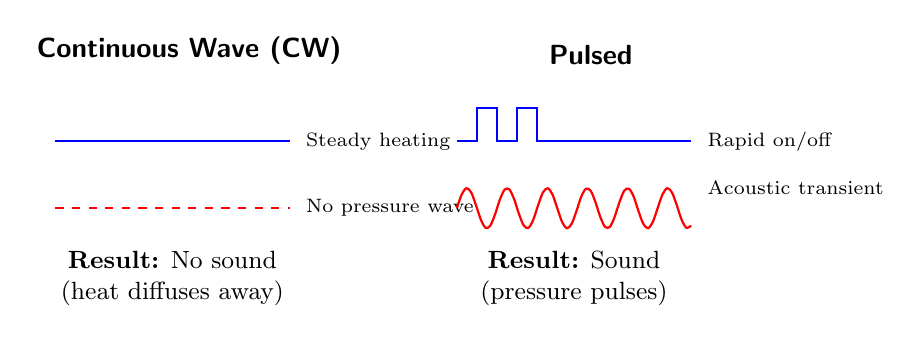
\begin{tikzpicture}[scale=0.85]
% CW case
\begin{scope}[shift={(0,0)}]
\node[above, font=\sffamily\bfseries] at (2,2.5) {Continuous Wave (CW)};
\draw[thick, blue] (0,1.5) -- (3.5,1.5);
\node[right, font=\scriptsize] at (3.6,1.5) {Steady heating};
\draw[thick, red, dashed] (0,0.5) -- (3.5,0.5);
\node[right, font=\scriptsize] at (3.6,0.5) {No pressure wave};
\node[below, font=\small, align=center] at (1.75,0) {\textbf{Result:} No sound\\(heat diffuses away)};
\end{scope}

% Pulsed case  
\begin{scope}[shift={(6,0)}]
\node[above, font=\sffamily\bfseries] at (2,2.5) {Pulsed};
\draw[thick, blue] (0,1.5) -- (0.3,1.5) -- (0.3,2) -- (0.6,2) -- (0.6,1.5) -- (0.9,1.5) -- (0.9,2) -- (1.2,2) -- (1.2,1.5) -- (3.5,1.5);
\node[right, font=\scriptsize] at (3.6,1.5) {Rapid on/off};
\draw[thick, red, smooth, samples=50, domain=0:3.5] plot (\x, {0.5 + 0.3*sin(360*\x/0.6)});
\node[right, font=\scriptsize] at (3.6,0.8) {Acoustic transient};
\node[below, font=\small, align=center] at (1.75,0) {\textbf{Result:} Sound\\(pressure pulses)};
\end{scope}
\end{tikzpicture}
\end{center}

\textbf{Key requirement:} Pulse duration $\tau$ must satisfy:
\begin{equation}
\tau < \tau_{\text{thermal}} \approx \frac{d^2}{4\kappa} \approx 1~\text{ms}
\label{eq:frey-pulse-req}
\end{equation}
where $d \sim$1~mm is the heated volume dimension and $\kappa \approx 1.4 \times 10^{-7}$~m$^2$/s is thermal diffusivity of tissue.

If pulses are too long, heat diffuses before expansion can launch an acoustic wave.

\section{Experimental Evidence}

\subsection{Human Psychophysical Studies}

\subsubsection{Threshold Measurements (Guy et al., 1975)}

Systematic studies established the frequency dependence and sensitivity thresholds:

\begin{center}
\begin{tabular}{@{}lcl@{}}
\toprule
\textbf{Frequency} & \textbf{Threshold} & \textbf{Notes} \\
\midrule
200~MHz & 100~$\mu$J/cm$^2$ & Poor penetration \\
915~MHz & 15~$\mu$J/cm$^2$ & Good penetration \\
\textbf{2.45~GHz} & \textbf{3--5~$\mu$J/cm$^2$} & \textbf{Peak sensitivity} \\
10~GHz & 30~$\mu$J/cm$^2$ & Surface absorption \\
\bottomrule
\end{tabular}
\end{center}

\textbf{Peak sensitivity at 2.45~GHz} coincides with maximum brain absorption (optimal balance between penetration and absorption).

\subsubsection{Perceived Sound Characteristics}

The perceived auditory sensation depends on pulse parameters:

\begin{itemize}
\item \textbf{Single pulse:} Sharp ``click'' or ``tap''
\item \textbf{10--100~pps:} Low-frequency ``buzz'' or ``hum''
\item \textbf{1000~pps:} Clear audible tone at 1~kHz
\item \textbf{$>$10~kHz PRF:} High-pitched whistle
\item \textbf{CW exposure:} No sound perception (even at high power)
\end{itemize}

\textbf{Critical finding:} Perceived frequency equals pulse repetition rate, \emph{not} the microwave carrier frequency.

\subsubsection{Evidence from Deaf Subjects}

\begin{center}
\begin{tabular}{@{}ll@{}}
\toprule
\textbf{Condition} & \textbf{Frey Effect Perception} \\
\midrule
Normal hearing & Yes \\
Conductive deafness (middle ear damage) & \textbf{Yes} (bypasses middle ear) \\
Sensorineural deafness (cochlear damage) & \textbf{No} (requires intact cochlea) \\
\bottomrule
\end{tabular}
\end{center}

This confirms the effect originates in the \textbf{cochlea}, not from direct neural stimulation.

\subsection{Animal Electrophysiology}

\subsubsection{Cochlear Microphonics (Elder \& Chou, 2003)}

Direct electrical recordings from guinea pig cochleae demonstrated:
\begin{itemize}
\item Microelectrode insertion into cochlea
\item Pulsed microwave exposure $\rightarrow$ electrical potentials matching PRF
\item Signal amplitude proportional to microwave pulse energy
\item \textbf{Cochlear ablation:} Effect completely abolished
\end{itemize}

\textbf{Conclusion:} Unambiguous evidence for cochlear transduction, not neural artifact.

\subsubsection{Auditory Brainstem Response (ABR)}

EEG-like measurements of auditory pathway activity showed:
\begin{itemize}
\item Pulsed microwaves evoke ABR waveforms similar to acoustic clicks
\item Latency consistent with cochlear origin ($\sim$2--5~ms)
\item No response in animals with destroyed cochleae
\end{itemize}

\subsection{Theoretical Validation}

\textbf{Lin's thermoelastic theory (1978--1980):}
\begin{itemize}
\item Predicted thresholds within factor of 2--3 of measured values
\item Explained frequency dependence based on penetration depth
\item Accounted for pulse width and PRF dependencies
\end{itemize}

\textbf{Foster \& Finch (1974):} Calculated pressure wave amplitudes consistent with psychophysical data.

\begin{keyconcept}
The thermoelastic mechanism is \textbf{firmly established} as the physical basis for the Frey effect. No alternative explanations (direct neural stimulation, equipment artifacts, etc.) are consistent with the comprehensive experimental evidence.
\end{keyconcept}

\section{Parameter Dependencies}

\subsection{Carrier Frequency}

The microwave carrier frequency determines penetration depth and absorption:

\begin{center}
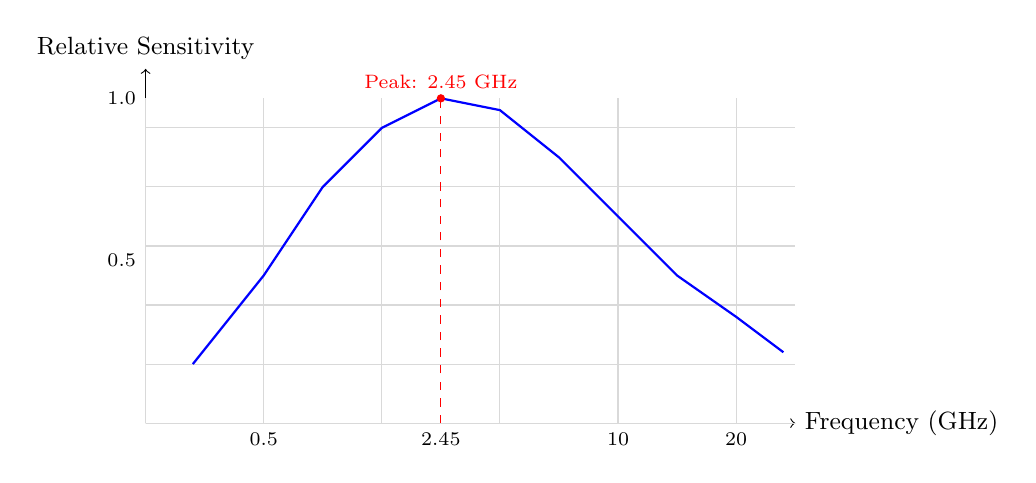
\begin{tikzpicture}[scale=0.75]
% Draw axes
\draw[->] (0,0) -- (11,0) node[right, font=\small] {Frequency (GHz)};
\draw[->] (0,0) -- (0,6) node[above, font=\small] {Relative Sensitivity};

% Add grid
\foreach \x in {0,2,4,6,8,10} {
  \draw[gray!30] (\x,0) -- (\x,5.5);
}
\foreach \y in {0,1,2,3,4,5} {
  \draw[gray!30] (0,\y) -- (11,\y);
}

% Draw sensitivity curve (Gaussian-like peaked at 2.45 GHz)
\draw[thick, blue, smooth] 
  (0.8,1) -- (2,2.5) -- (3,4) -- (4,5) -- (5,5.5) -- (6,5.3) -- (7,4.5) -- (8,3.5) -- (9,2.5) -- (10,1.8) -- (10.8,1.2);

% Mark peak at 2.45 GHz (around x=5)
\draw[dashed, red] (5,0) -- (5,5.5) node[above, font=\scriptsize] {Peak: 2.45~GHz};
\fill[red] (5,5.5) circle (2pt);

% Add tick labels
\node[below, font=\scriptsize] at (2,0) {0.5};
\node[below, font=\scriptsize] at (5,0) {2.45};
\node[below, font=\scriptsize] at (8,0) {10};
\node[below, font=\scriptsize] at (10,0) {20};
\node[left, font=\scriptsize] at (0,2.75) {0.5};
\node[left, font=\scriptsize] at (0,5.5) {1.0};
\end{tikzpicture}
\end{center}

\textbf{Frequency regimes:}
\begin{itemize}
\item \textbf{$<$100~MHz:} Deep penetration but low brain absorption $\rightarrow$ weak effect
\item \textbf{1--10~GHz:} Optimal range (adequate penetration + good absorption)
\item \textbf{$>$30~GHz:} Surface absorption only; doesn't reach cochlea
\end{itemize}

\subsection{Pulse Duration}

\begin{equation}
\text{Optimal range: } \tau \approx 1\text{--}100~\mu\text{s}
\label{eq:frey-pulse-width}
\end{equation}

\textbf{Trade-offs:}
\begin{itemize}
\item \textbf{Too short ($<$1~$\mu$s):} Insufficient energy deposition $\rightarrow$ weak pressure
\item \textbf{Too long ($>$1~ms):} Heat diffuses before expansion $\rightarrow$ inefficient transduction
\end{itemize}

\subsection{Pulse Repetition Frequency (PRF)}

\textbf{PRF directly determines perceived pitch:}

\begin{center}
\begin{tabular}{@{}ll@{}}
\toprule
\textbf{PRF} & \textbf{Perceived Sound} \\
\midrule
$<$20~Hz & Individual clicks (infrasound) \\
20--100~Hz & Low-frequency hum/buzz \\
100--1000~Hz & Clear audible tone \\
1--10~kHz & Musical pitch range \\
10--20~kHz & High-pitched whistle \\
$>$20~kHz & Ultrasound (typically not perceived) \\
\bottomrule
\end{tabular}
\end{center}

\begin{calloutbox}{Example: Speech Transmission}
By modulating the PRF to follow speech formants (fundamental frequency 100--300~Hz, harmonics up to 4~kHz), researchers have transmitted intelligible speech directly to a subject's auditory system---the so-called ``voice-to-skull'' effect. Intelligibility is limited by PRF bandwidth constraints.
\end{calloutbox}

\subsection{Peak Power vs. Average Power}

\textbf{Critical insight:} The effect depends on \textbf{peak pulse energy}, not time-averaged power.

\begin{equation}
\text{Average power: } P_{\text{avg}} = P_{\text{peak}} \times \tau \times \text{PRF}
\label{eq:frey-avg-power}
\end{equation}

\textbf{Example calculation:}
\begin{itemize}
\item Peak power: $P_{\text{peak}} = 1$~kW
\item Pulse width: $\tau = 1$~$\mu$s
\item PRF: 100~pps
\item Duty cycle: $1 \times 10^{-6} \times 100 = 10^{-4}$ (0.01\%)
\item Average power: $P_{\text{avg}} = 1000 \times 10^{-6} \times 100 = 0.1$~W
\end{itemize}

\begin{warningbox}
\textbf{Safety implication:} Time-averaged power density can be well below regulatory limits while peak pulse intensity is sufficient to cause auditory perception. Safety standards based solely on average power may not account for pulsed exposure effects.
\end{warningbox}

\section{Worked Example: Radar Installation Exposure}

\textbf{Scenario:} Personnel working near a ground surveillance radar experience auditory sensations. Determine if this is consistent with the Frey effect.

\subsection*{Given Parameters}

\begin{tabular}{@{}ll@{}}
Radar frequency & $f_c = 10$~GHz (X-band) \\
Peak power & $P_{\text{peak}} = 500$~kW \\
Pulse width & $\tau = 2$~$\mu$s \\
PRF & 500~pps \\
Antenna gain & $G_t = 35$~dBi = 3162 (linear) \\
Distance & $d = 50$~m (side lobe exposure) \\
Side lobe level & $-20$~dB relative to main beam \\
\end{tabular}

\subsection*{Step 1: Effective Radiated Power}

Side lobe gain (linear):
\begin{equation}
G_{\text{side}} = G_t \times 10^{-20/10} = 3162 \times 0.01 = 31.62
\end{equation}

Effective isotropic radiated power (EIRP):
\begin{equation}
\text{EIRP}_{\text{side}} = P_{\text{peak}} \times G_{\text{side}} = 500 \times 10^3 \times 31.62 = 15.81~\text{MW}
\end{equation}

\subsection*{Step 2: Power Density at Personnel Location}

Free-space power density:
\begin{equation}
S = \frac{\text{EIRP}}{4\pi d^2} = \frac{15.81 \times 10^6}{4\pi (50)^2} = 503~\text{W/m}^2 = 50.3~\text{mW/cm}^2
\end{equation}

\subsection*{Step 3: Energy Fluence per Pulse}

\begin{equation}
E_f = S \times \tau = 50.3 \times 10^{-3} \times 2 \times 10^{-6} = 1.01 \times 10^{-7}~\text{J/cm}^2 = 0.10~\mu\text{J/cm}^2
\end{equation}

\subsection*{Step 4: Compare to Threshold}

\begin{center}
\begin{tabular}{@{}ll@{}}
Calculated energy fluence & $0.10$~$\mu$J/cm$^2$ \\
Frey effect threshold (10~GHz) & $\sim$30~$\mu$J/cm$^2$ \\
\textbf{Ratio} & \textbf{0.003 (300$\times$ below threshold)} \\
\end{tabular}
\end{center}

\subsection*{Step 5: Perceived Frequency}

If exposure were at threshold level, the perceived sound would be:
\begin{equation}
f_{\text{perceived}} = \text{PRF} = 500~\text{Hz} \quad \text{(mid-frequency tone)}
\end{equation}

\begin{calloutbox}[colback=black!8!white,colframe=black]{Conclusion}
\textbf{Result:} The calculated exposure is \textbf{300$\times$ below} the Frey effect threshold at 10~GHz. Personnel would \textbf{not} experience auditory sensations under these conditions.

\textbf{To reach threshold:} Would require:
\begin{itemize}
\item Moving to $d \approx 3$~m (300$\times$ closer), or
\item Direct main beam exposure (not side lobe), or
\item Higher peak power
\end{itemize}

\textbf{Safety note:} Even though Frey effect won't occur, the power density of 50~mW/cm$^2$ \textbf{exceeds} IEEE occupational exposure limits (10~mW/cm$^2$). Thermal hazards remain a concern.
\end{calloutbox}

\section{Safety Considerations}
\label{sec:frey-safety}

\subsection{Exposure Limits and Regulatory Standards}

\textbf{IEEE/ICNIRP RF exposure guidelines} (based on thermal effects):

\begin{center}
\begin{tabular}{@{}ll@{}}
\toprule
\textbf{Population} & \textbf{Limit (1--10~GHz)} \\
\midrule
Occupational & 10~mW/cm$^2$ (6-minute average) \\
General public & 2~mW/cm$^2$ (30-minute average) \\
\bottomrule
\end{tabular}
\end{center}

\textbf{Frey effect threshold:}
\begin{itemize}
\item Energy fluence: $\sim$5~$\mu$J/cm$^2$ per pulse
\item For $\tau = 1$~$\mu$s, PRF = 100~pps:
\end{itemize}

\begin{equation}
P_{\text{avg}} = \frac{E_f \times \text{PRF}}{10^{-3}} = \frac{5 \times 10^{-6} \times 100}{10^{-3}} = 0.5~\text{mW/cm}^2
\end{equation}

\begin{keyconcept}
The Frey effect can occur at exposures \textbf{well below} thermal safety limits (factor of 4--20$\times$ lower). Current RF safety standards, based primarily on preventing thermal damage, do not explicitly address pulsed exposure effects like microwave hearing.
\end{keyconcept}

\subsection{Health Effects}

\subsubsection{Acute Effects}
\begin{itemize}
\item \textbf{Primary:} Auditory perception (transient, fully reversible)
\item \textbf{Secondary:} Annoyance, distraction, startle response
\item \textbf{No tissue damage} at threshold levels
\item Equivalent SPL: $\sim$60--80~dB (moderate loudness, not hazardous)
\end{itemize}

\subsubsection{Chronic Effects}
\begin{itemize}
\item No documented long-term health effects from brief, threshold-level exposures
\item Prolonged high-intensity exposure \emph{could} theoretically cause cochlear damage (analogous to acoustic trauma)
\item No epidemiological evidence of adverse effects in occupationally exposed populations
\end{itemize}

\begin{calloutbox}{Comparison to Acoustic Sound}
Frey effect pressure waves at threshold correspond to approximately 70~dB SPL---the loudness of normal conversation. This is far below levels that cause hearing damage ($>$85~dB for prolonged exposure, $>$120~dB for acute trauma).
\end{calloutbox}

\section{Applications}

\subsection{Non-Lethal Deterrent Systems}

\textbf{Concept:} Direct pulsed microwaves at personnel to induce disorienting auditory sensations or transmit warning messages (``voice-to-skull'' effect).

\textbf{Advantages:}
\begin{itemize}
\item[\checkmark] No physical projectile or contact required
\item[\checkmark] Fully reversible, non-injurious effect
\item[\checkmark] Can encode complex information (speech patterns)
\item[\checkmark] Penetrates clothing, protective gear
\end{itemize}

\textbf{Challenges:}
\begin{itemize}
\item[\texttimes] High peak power (kW) requires bulky equipment
\item[\texttimes] Line-of-sight only; no through-wall capability at GHz frequencies
\item[\texttimes] Significant ethical concerns regarding psychological impact
\item[\texttimes] Potential for misuse or perception as ``mind control''
\end{itemize}

\textbf{Status:} Prototype systems developed (e.g., U.S. military MEDUSA project, 2008). Operational deployment remains unclear due to ethical and policy constraints.

\subsection{Communication Systems}

\textbf{Covert/Directional Audio:}
\begin{itemize}
\item Highly directional transmission (only target individual hears)
\item Potential for specialized military/intelligence applications
\item Speech intelligibility limited by PRF bandwidth ($\sim$10~kHz maximum)
\item Requires precise beam focusing and stationary target
\end{itemize}

\textbf{Practical limitations:}
\begin{itemize}
\item Short range (meters to tens of meters for portable systems)
\item Cannot compete with conventional communication methods for most applications
\item Beam steering complexity for moving targets
\end{itemize}

\subsection{Medical Applications (Speculative)}

\textbf{Original hypothesis:} Bypass damaged middle ear for hearing restoration.

\textbf{Reality:} The Frey effect \emph{requires} intact cochlear function. Patients with sensorineural hearing loss (cochlear hair cell damage) cannot perceive the effect.

\textbf{Conclusion:} Cochlear implants (electrical stimulation) are far more effective and practical for hearing restoration.

\subsection{Neuroscience Research Tool}

\textbf{Potential:} Selective, non-invasive activation of auditory pathways for functional brain imaging (fMRI, PET).

\textbf{Status:} Not actively pursued due to:
\begin{itemize}
\item Ethical review barriers for human exposure studies
\item Availability of alternative acoustic stimulation methods
\item Difficulty controlling for potential confounds (thermal effects, EMI)
\end{itemize}

\begin{calloutbox}{Ethical Considerations}
Any application involving transmission of information directly to a person's auditory system raises significant ethical questions:
\begin{itemize}
\item Informed consent and autonomy
\item Potential for covert influence or harassment
\item Psychological impact of ``disembodied voices''
\item Military/intelligence use vs. civilian protection
\end{itemize}

Responsible development requires robust ethical frameworks and regulatory oversight.
\end{calloutbox}

\section{Comparison to Related Phenomena}

\subsection{Acoustic Heterodyning}
\label{subsec:frey-vs-heterodyning}

\textbf{Similarity:} Both create sound perception without a conventional acoustic source.

\textbf{Key difference:}
\begin{itemize}
\item \textbf{Acoustic heterodyning:} Two ultrasonic beams mix \emph{in air}, creating audible difference frequency
\item \textbf{Frey effect:} Electromagnetic-to-acoustic transduction \emph{in tissue}
\end{itemize}

See Chapter~\ref{ch:acoustic-heterodyning} for details on parametric acoustic arrays.

\subsection{THz Bioeffects}

\textbf{Question:} Can terahertz radiation (0.1--10~THz) produce a Frey-like effect?

\textbf{Answer:} \textbf{No.} Key differences:

\begin{center}
\begin{tabular}{@{}lll@{}}
\toprule
\textbf{Parameter} & \textbf{Microwaves (Frey)} & \textbf{THz} \\
\midrule
Frequency & 1--10~GHz & 100--10,000~GHz \\
Penetration depth & 1--3~cm & $<$1~mm \\
Reaches cochlea? & Yes & No (absorbed at skin) \\
Effect mechanism & Volumetric heating & Surface heating only \\
\bottomrule
\end{tabular}
\end{center}

See Chapter~\ref{ch:thz-bioeffects} for THz-tissue interactions.

\section{Controversies and Misconceptions}

\subsection{``Mind Control'' and Conspiracy Theories}

\textbf{Misconception:} The Frey effect enables thought implantation or behavioral control.

\textbf{Reality:}
\begin{itemize}
\item The effect produces only \textbf{auditory perception}---functionally equivalent to hearing via normal acoustic pathways
\item Cannot write information directly to memory or cognition centers
\item No different from listening to a voice through headphones
\item Recipient remains fully autonomous and aware
\end{itemize}

\begin{warningbox}
While the Frey effect cannot ``control minds,'' the ability to transmit sounds to an individual covertly does raise legitimate concerns about harassment, privacy invasion, and psychological manipulation through deception. These are \textbf{social/ethical issues}, not physics limitations.
\end{warningbox}

\subsection{``Havana Syndrome'' Speculation}

\textbf{Context:} Unexplained health incidents (2016--present) affecting U.S. and Canadian diplomats, characterized by:
\begin{itemize}
\item Sudden onset of pressure/pain sensations
\item Auditory phenomena (chirping, grinding sounds)
\item Persistent neurological symptoms
\item Cluster occurrence in specific locations
\end{itemize}

\textbf{Hypothesized explanations:}
\begin{enumerate}
\item Pulsed microwave exposure (Frey effect)
\item Ultrasonic weapons
\item Mass psychogenic illness
\item Environmental factors (pesticides, infectious agents)
\end{enumerate}

\textbf{Scientific assessment:}
\begin{itemize}
\item Mechanism remains \textbf{unproven}
\item Microwave explanation is \emph{plausible} but lacks direct evidence
\item Persistent symptoms not consistent with simple Frey effect (transient)
\item National Academy of Sciences report (2020): ``directed pulsed RF energy'' most consistent with acute symptoms
\end{itemize}

\subsection{5G, Cell Phones, and Wi-Fi}

\textbf{Question:} Can consumer wireless devices (5G towers, cell phones, Wi-Fi routers) cause Frey effect?

\textbf{Answer:} \textbf{No.} Multiple barriers:

\begin{center}
\begin{tabular}{@{}lll@{}}
\toprule
\textbf{Requirement} & \textbf{Frey Effect} & \textbf{Consumer Wireless} \\
\midrule
Signal type & Short pulses ($\mu$s) & CW or quasi-CW \\
Peak power & kW & mW (1 million$\times$ less) \\
Energy/pulse & $\mu$J/cm$^2$ & $\ll$nJ/cm$^2$ \\
Frequency & 1--10~GHz optimal & Sub-optimal (e.g., 28~GHz for mmWave 5G) \\
\bottomrule
\end{tabular}
\end{center}

\textbf{Conclusion:} Consumer devices lack both the pulse structure and power levels required. Claims of Frey-effect-related symptoms from cell phones/5G are not scientifically supported.

\section{Summary}

\begin{center}
\begin{tabular}{@{}ll@{}}
\toprule
\textbf{Parameter} & \textbf{Value/Description} \\
\midrule
Effect type & Thermoelastic EM-to-acoustic transduction \\
Discovery & Allan Frey, 1962 \\
Carrier frequency & 1--10~GHz (optimal: 2.45~GHz) \\
Pulse requirement & Yes (1--100~$\mu$s duration) \\
PRF range & 20~Hz--20~kHz (audible range) \\
Energy threshold & 1--10~$\mu$J/cm$^2$ per pulse \\
Temperature rise & $\sim$10$^{-6}$~K (negligible) \\
Pressure amplitude & $\sim$0.1--1~Pa (60--80~dB SPL) \\
Mechanism & Rapid heating $\rightarrow$ expansion $\rightarrow$ acoustic wave \\
Cochlear requirement & Yes (intact hair cells essential) \\
Safety & Below thermal limits; transient, reversible \\
Applications & Non-lethal deterrents, specialized comms \\
Misconceptions & Cannot control thoughts or implant information \\
\bottomrule
\end{tabular}
\end{center}

\begin{keyconcept}
The Frey microwave auditory effect is a well-established phenomenon in which pulsed microwave radiation generates audible sensations through thermoelastic pressure wave generation in brain tissue. The effect demonstrates a fascinating example of electromagnetic-biological coupling but does not pose health risks at threshold exposure levels nor enable ``mind control'' as sometimes speculated.
\end{keyconcept}

\section{References}

\subsection*{Original Discovery}

\begin{enumerate}
\item \textbf{Frey, A.H.} ``Auditory System Response to Radio Frequency Energy.'' \emph{Journal of Applied Physiology} 17(4):689--692 (1962). DOI: 10.1152/jappl.1962.17.4.689

\textit{First systematic report of microwave hearing phenomenon.}
\end{enumerate}

\subsection*{Mechanism and Theory}

\begin{enumerate}
\setcounter{enumi}{1}
\item \textbf{Lin, J.C.} ``Microwave Auditory Effects and Applications.'' \emph{Proceedings of the IEEE} 68(1):67--73 (1980). DOI: 10.1109/PROC.1980.11581

\textit{Definitive review of thermoelastic theory and quantitative predictions.}

\item \textbf{Foster, K.R. \& Finch, E.D.} ``Microwave Hearing: Evidence for Thermoacoustic Auditory Stimulation by Pulsed Microwaves.'' \emph{Science} 185(4147):256--258 (1974). DOI: 10.1126/science.185.4147.256

\textit{Theoretical calculations of pressure wave amplitudes.}
\end{enumerate}

\subsection*{Experimental Confirmation}

\begin{enumerate}
\setcounter{enumi}{3}
\item \textbf{Guy, A.W., Chou, C.K., Lin, J.C., \& Christensen, D.} ``Microwave-Induced Acoustic Effects in Mammalian Auditory Systems and Physical Materials.'' \emph{Radio Science} 10(2):109--119 (1975). DOI: 10.1029/RS010i002p00109

\textit{Comprehensive psychophysical threshold measurements in humans.}

\item \textbf{Elder, J.A. \& Chou, C.K.} ``Auditory Response to Pulsed Radiofrequency Energy.'' \emph{Bioelectromagnetics} 24(S6):S162--S173 (2003). DOI: 10.1002/bem.10163

\textit{Direct cochlear microphonic recordings demonstrating transduction mechanism.}
\end{enumerate}

\subsection*{Reviews and Safety Assessments}

\begin{enumerate}
\setcounter{enumi}{5}
\item \textbf{Lin, J.C. \& Gandhi, O.P.} ``Computational Methods for Predicting Field Intensity and Temperature Change.'' \emph{IEEE Transactions on Antennas and Propagation} 44(11):1413--1421 (1996). DOI: 10.1109/8.542070

\textit{Safety analysis and exposure assessment.}

\item \textbf{Elder, J.A.} ``Survival and Cancer in Laboratory Mammals Exposed to Radiofrequency Energy.'' \emph{Health Physics} 83(5):580--583 (2002). DOI: 10.1097/00004032-200211000-00002

\textit{Comprehensive review of biological effects and safety.}

\item \textbf{National Academies of Sciences, Engineering, and Medicine.} \emph{An Assessment of Illness in U.S. Government Employees and Their Families at Overseas Embassies.} Washington, DC: The National Academies Press (2020). DOI: 10.17226/25889

\textit{Scientific evaluation of ``Havana Syndrome'' incidents; considers directed RF energy.}
\end{enumerate}

\section{Further Reading}

\begin{itemize}
\item \textbf{Chapter \ref{ch:non-linear-biological-demodulation}:} Non-Linear Biological Demodulation---broader context of EM-biology interactions

\item \textbf{Chapter \ref{ch:acoustic-heterodyning}:} Acoustic Heterodyning---parametric acoustic arrays (different mechanism, similar perceptual result)

\item \textbf{Chapter \ref{ch:intermodulation-biology}:} Intermodulation Distortion in Biology---nonlinear mixing in biological systems

\item \textbf{Chapter \ref{ch:thz-bioeffects}:} THz Bioeffects---comparison to higher-frequency radiation interactions

\item \textbf{Chapter \ref{ch:biophysical-coupling}:} Biophysical Coupling Mechanisms---general framework for EM field interactions with tissue

\item \textbf{Chapter \ref{ch:rf-safety}:} RF Safety Standards---regulatory context and exposure limits
\end{itemize}
